%!TEX output_directory = aux_dir
\documentclass[../SommerstjernerA4.tex]{subfiles}

\begin{document}
\section{Planeter}
Om sommeren 2017 er det i hovedsak to planeter som er synlige: Jupiter om kvelden og Venus om morgenen.
\subsection{Jupiter}
Jupiter er synlig rett etter solnedgang i sør-vest. Dessverre beveger den seg nærmere solen i løpet av sommeren, så den blir vanskeligere å se.

Jupiter er den største planeten i solsystemet, og har fire store måner (Europa, Ganymedes, Callisto og Io) som det er mye å snakke om. De er også relativt enkle å se i virkeligheten; du trenger bare en vanlig kikkert eller en god zoomlinse. Hvis du er heldig kan du også få se stripene på Jupiter.

Det er mye man kan snakke om på Jupiter: Stormene, månene, fargebåndene som av og til forsvinner, og så videre.

Akkurat nå har Jupiter besøk av romsonden Juno, som gjør målinger av Jupiters atmosfære, gravitasjon- og magnetfelt. Juno tar også mange flotte bilder av stormene på Jupiter.

\begin{figure}[bh]
\centering
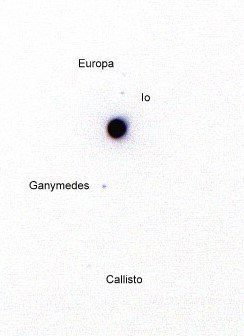
\includegraphics{negativ-jupiter}
\caption{Negativt bilde av Jupiter og de fire galileiske månene. Bilde tatt i oktober 2010.}
\end{figure}

\subsection{Venus}
Venus er synlig hele sommeren rett før soloppgang i øst. Den blir litt enklere å se utover sommeren, men du må opp veldig tidlig.

Jeg syntes selv at Venus er en av de fineste tingene å se på himmelen fordi den er så utrolig lys. Venus er det tredje lyseste objektet på himmelen etter solen og månen. Dersom man har kikkert kan man observere faser på Venus som på månen. 
\end{document}